
%(BEGIN_QUESTION)
% Copyright 2006, Tony R. Kuphaldt, released under the Creative Commons Attribution License (v 1.0)
% This means you may do almost anything with this work of mine, so long as you give me proper credit

Suppose we tried to build a very simple gas chromatograph, where the output voltage of the flame ionization detector (FID) connects directly to an analog chart recorder:

$$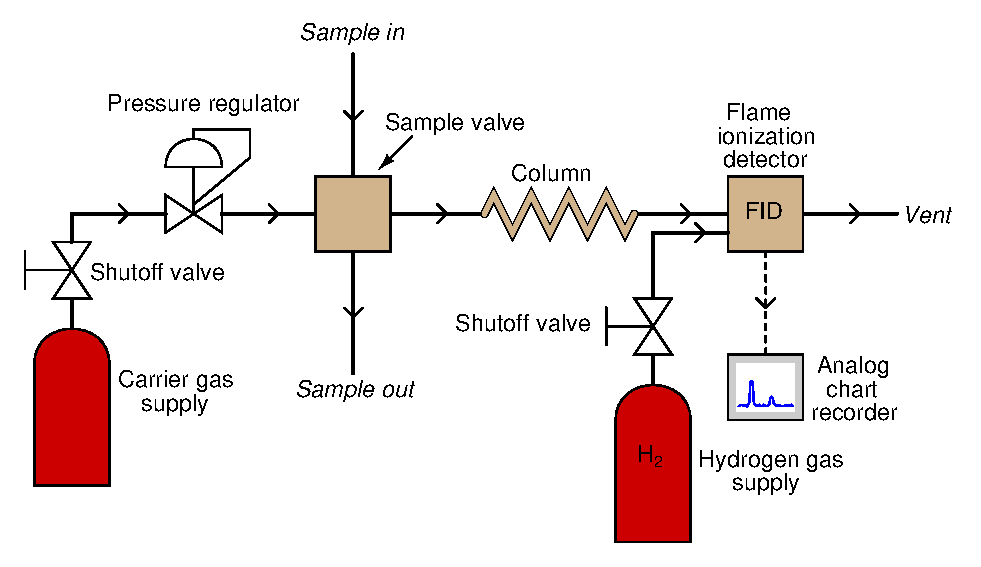
\includegraphics[width=15.5cm]{i01356x01.eps}$$

This chart recorder will produce a chromatogram, but it will be a rather strange one: we will not be able to accurately interpret it in its raw form.  The height of the peaks on this chromatogram will {\it not} necessarily indicate the flow rates of the separated components exiting the column.

Explain why this chromatogram will not be accurate as displayed, and explain what is required to correct it (i.e. how modern process chromatographs solve this problem).

\underbar{file i01356}
%(END_QUESTION)





%(BEGIN_ANSWER)

The problem is that the different compounds exiting the chromatograph column will not all ionize equally in a flame.  This means the heights of the chromatogram peaks vary with component flow rate {\it and} with relative ionization ability.
 
\vskip 10pt

This is a fundamental problem for all chromatographs, regardless of detector type.  The solution to the problem is to ``program'' the gain of the detector according to what component is expected to exit the column at any given time.  This by itself makes it clear why all process chromatographs are microprocessor-controlled.

%(END_ANSWER)





%(BEGIN_NOTES)


%INDEX% Measurement, analytical: chromatography

%(END_NOTES)


